\documentclass[aspectratio=169,11pt]{beamer}

% Theme and colors
\usetheme{Madrid}
\usecolortheme{whale}
\setbeamertemplate{navigation symbols}{}
\setbeamertemplate{footline}[frame number]

% Packages
\usepackage[utf8]{inputenc}
\usepackage[T1]{fontenc}
\usepackage{graphicx}
\usepackage{booktabs}
\usepackage{amsmath}
\usepackage{hyperref}
\usepackage{tikz}
\usetikzlibrary{shapes,arrows,positioning,calc,fit,backgrounds,decorations.pathmorphing,patterns}
\usepackage{siunitx}
\usepackage{xcolor}

% Custom colors
\definecolor{questionbg}{RGB}{255,248,220}
\definecolor{questionborder}{RGB}{255,193,7}

% Title information
\title[EECE5155 -- Module 4 Part 4]{Wireless Communication Standards for IoT}
\subtitle{Module 4 Part 4: From PAN to LPWAN}
\author{Eduardo Baena}
\date{Spring 2026}
\institute{Northeastern University\\Department of Electrical and Computer Engineering\\
\texttt{e.baena@northeastern.edu}}

\begin{document}

% Title slide
\begin{frame}
    \titlepage
    \vspace{-1cm}
    \begin{center}
        \textbf{EECE5155: Wireless Sensor Networks and the Internet of Things}
    \end{center}
\end{frame}

% Learning Objectives
\begin{frame}{Learning Objectives}
    \textbf{By the end of this module, you should be able to:}
    
    \vspace{0.5cm}
    \begin{enumerate}
        \item \textbf{Describe} the PHY and MAC layer mechanisms of major IoT wireless standards
        \item \textbf{Explain} the architectural differences between PAN, LAN, and LPWAN technologies
        \item \textbf{Compare} IEEE 802.15.4, Bluetooth/BLE, Wi-Fi, and LPWAN at the protocol level
        \item \textbf{Identify} which standard features matter for specific IoT use cases
        \item \textbf{Evaluate} emerging standards (Bluetooth 6.0, Wi-Fi 7, Matter/Thread, 5G RedCap)
    \end{enumerate}
    
    \vspace{0.3cm}
    \begin{alertblock}{Prerequisite}
        This module assumes you have completed Module 4 Parts 1--3 (energy models, protocol overview, link layer fundamentals).
    \end{alertblock}
\end{frame}

% Outline
\begin{frame}{Outline}
    \begin{columns}
        \column{0.5\textwidth}
        \begin{enumerate}
            \item \textbf{IEEE 802.15.4}
            \begin{itemize}
                \item PHY and MAC
                \item Superframe structure
                \item ZigBee, Thread, Matter
            \end{itemize}
            
            \item \textbf{Bluetooth / BLE}
            \begin{itemize}
                \item Classic architecture
                \item BLE 5.x for IoT
                \item Bluetooth 6.0 Channel Sounding
            \end{itemize}
            
            \item \textbf{IEEE 802.11 (Wi-Fi)}
            \begin{itemize}
                \item Protocol stack and evolution
                \item CSMA/CA and RTS/CTS
                \item 802.11ah (HaLow) and Wi-Fi 7
            \end{itemize}
        \end{enumerate}
        
        \column{0.5\textwidth}
        \begin{enumerate}
            \setcounter{enumi}{3}
            \item \textbf{Cellular IoT}
            \begin{itemize}
                \item NB-IoT and LTE-M
                \item 5G RedCap / eRedCap
            \end{itemize}
            
            \item \textbf{LPWAN Technologies}
            \begin{itemize}
                \item LoRaWAN: modulation, classes, security
                \item Sigfox / 0G Technology
            \end{itemize}
            
            \item \textbf{Technology Classification}
            \begin{itemize}
                \item Short-range vs long-range
                \item Licensed vs unlicensed
                \item The LPWAN sweet spot
            \end{itemize}
        \end{enumerate}
    \end{columns}
\end{frame}

%==============================================================================
\section{IEEE 802.15.4}
%==============================================================================

\begin{frame}{IEEE 802.15.4: The Foundation of IoT Mesh}
    \textbf{IEEE 802.15.4 defines PHY and MAC for Low-Rate Wireless Personal Area Networks (LR-WPAN).}
    
    \vspace{0.3cm}
    \begin{columns}
        \column{0.5\textwidth}
        \textbf{Key Characteristics:}
        \begin{itemize}
            \item Data rates: 20, 40, 250 kbps
            \item Frequencies: 868 MHz, 915 MHz, 2.4 GHz
            \item Range: 10--100 m (typical)
            \item Star and peer-to-peer topologies
            \item Up to 65,536 nodes per network
        \end{itemize}
        
        \column{0.5\textwidth}
        \textbf{Two device types:}
        \begin{itemize}
            \item \textbf{FFD} (Full Function Device):
            \begin{itemize}
                \item Can be PAN coordinator
                \item Talks to any device
            \end{itemize}
            \item \textbf{RFD} (Reduced Function Device):
            \begin{itemize}
                \item Talks only to FFDs
                \item Simpler, lower cost
            \end{itemize}
        \end{itemize}
    \end{columns}
    
    \vspace{0.3cm}
    \begin{exampleblock}{Why This Matters}
        802.15.4 is the \textbf{PHY/MAC foundation} for ZigBee, Thread, Matter, 6LoWPAN, and many industrial IoT stacks. Understanding it means understanding the base layer of IoT mesh networking.
    \end{exampleblock}
\end{frame}

\begin{frame}{IEEE 802.15.4: Superframe Structure}
    \textbf{When beacons are enabled, the PAN coordinator defines a superframe:}
    
    \vspace{0.3cm}
    \begin{center}
    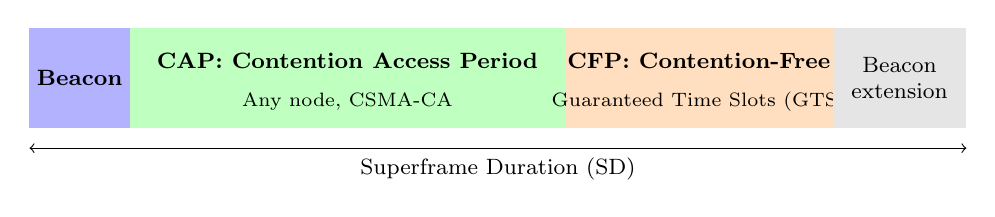
\begin{tikzpicture}[scale=0.85, every node/.style={font=\footnotesize}]
        % Beacon
        \fill[blue!30] (0,0) rectangle (1.5,1.5);
        \node[align=center] at (0.75,0.75) {\textbf{Beacon}};
        % CAP
        \fill[green!25] (1.5,0) rectangle (8,1.5);
        \node[align=center] at (4.75,1.0) {\textbf{CAP: Contention Access Period}};
        \node[align=center, font=\scriptsize] at (4.75,0.4) {Any node, CSMA-CA};
        % CFP
        \fill[orange!25] (8,0) rectangle (12,1.5);
        \node[align=center] at (10,1.0) {\textbf{CFP: Contention-Free}};
        \node[align=center, font=\scriptsize] at (10,0.4) {Guaranteed Time Slots (GTS)};
        % Beacon extension
        \fill[gray!20] (12,0) rectangle (14,1.5);
        \node[align=center] at (13,0.75) {Beacon\\extension};
        % Labels
        \draw[<->] (0,-0.3) -- (14,-0.3) node[midway,below] {Superframe Duration (SD)};
    \end{tikzpicture}
    \end{center}
    
    \vspace{0.2cm}
    \begin{itemize}
        \item \textbf{Beacon:} Transmitted by PAN coordinator. Contains network info, frame structure, pending messages.
        \item \textbf{CAP:} Any node accesses using slotted CSMA-CA.
        \item \textbf{CFP:} Reserved Guaranteed Time Slots for nodes needing deterministic bandwidth.
    \end{itemize}
    
    \begin{alertblock}{Design Tradeoff}
        Beacons enable synchronization and GTS but add overhead. Non-beacon mode uses unslotted CSMA-CA (simpler, but no guaranteed bandwidth).
    \end{alertblock}
\end{frame}

\begin{frame}{IEEE 802.15.4: Frame Formats}
    \textbf{General MAC Frame:}
    
    \vspace{0.2cm}
    \begin{center}
    \footnotesize
    \begin{tabular}{|c|c|c|c|c|c|c|}
        \hline
        \textbf{Frame} & \textbf{Seq.} & \textbf{Dest.} & \textbf{Dest.} & \textbf{Source} & \textbf{Source} & \textbf{Frame} \\
        \textbf{Control} & \textbf{Number} & \textbf{PAN ID} & \textbf{Address} & \textbf{PAN ID} & \textbf{Address} & \textbf{Check} \\
        \hline
        2 oct & 1 oct & 0/2 oct & 0/2/8 oct & 0/2 oct & 0/2/8 oct & 2 oct \\
        \hline
    \end{tabular}
    \normalsize
    \end{center}
    
    \vspace{0.2cm}
    \textbf{Frame Control field (16 bits):}
    \begin{itemize}
        \item Bits 0--2: Frame type (beacon, data, ACK, MAC command)
        \item Bit 3: Security enabled
        \item Bit 4: Frame pending
        \item Bit 5: ACK request
    \end{itemize}
    
    \vspace{0.2cm}
    \textbf{PHY Frame wraps MAC frame:}
    \begin{center}
    \footnotesize
    \begin{tabular}{|c|c|c|c|}
        \hline
        \textbf{Preamble} & \textbf{SFD} & \textbf{PHY Hdr} & \textbf{PSDU (MAC frame)} \\
        \hline
        4 bytes (sync) & 1 byte & 1 byte (length) & 0--127 bytes \\
        \hline
    \end{tabular}
    \normalsize
    \end{center}
    
    Max payload: 127 bytes $-$ overhead $\approx$ \textbf{104 bytes} useful data.
\end{frame}

\begin{frame}{From 802.15.4 to ZigBee, Thread, and Matter}
    \textbf{IEEE 802.15.4 defines only PHY and MAC. Higher layers are defined by different alliances:}
    
    \vspace{0.3cm}
    \begin{center}
    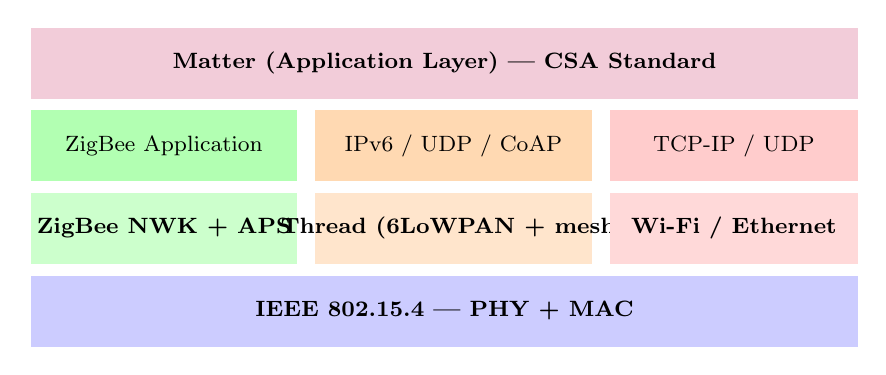
\begin{tikzpicture}[scale=0.75, every node/.style={font=\footnotesize}]
        % Base layer
        \fill[blue!20] (0,0) rectangle (14,1.2);
        \node at (7,0.6) {\textbf{IEEE 802.15.4 --- PHY + MAC}};
        % ZigBee stack
        \fill[green!20] (0,1.4) rectangle (4.5,2.6);
        \node at (2.25,2.0) {\textbf{ZigBee NWK + APS}};
        \fill[green!30] (0,2.8) rectangle (4.5,4.0);
        \node at (2.25,3.4) {ZigBee Application};
        % Thread stack
        \fill[orange!20] (4.8,1.4) rectangle (9.5,2.6);
        \node at (7.15,2.0) {\textbf{Thread (6LoWPAN + mesh)}};
        \fill[orange!30] (4.8,2.8) rectangle (9.5,4.0);
        \node at (7.15,3.4) {IPv6 / UDP / CoAP};
        % Matter
        \fill[purple!20] (0,4.2) rectangle (14,5.4);
        \node at (7,4.8) {\textbf{Matter (Application Layer) --- CSA Standard}};
        % Wi-Fi path
        \fill[red!15] (9.8,1.4) rectangle (14,2.6);
        \node at (11.9,2.0) {\textbf{Wi-Fi / Ethernet}};
        \fill[red!20] (9.8,2.8) rectangle (14,4.0);
        \node at (11.9,3.4) {TCP-IP / UDP};
    \end{tikzpicture}
    \end{center}
    
    \vspace{0.2cm}
    \begin{columns}
        \column{0.33\textwidth}
        \textbf{ZigBee 3.0:}
        \begin{itemize}
            \item Proprietary mesh NWK
            \item 250 kbps, 100m
            \item Philips Hue, SmartThings
        \end{itemize}
        
        \column{0.33\textwidth}
        \textbf{Thread 1.4 (2024):}
        \begin{itemize}
            \item IPv6-native mesh
            \item Credential sharing
            \item Apple, Google, Amazon
        \end{itemize}
        
        \column{0.33\textwidth}
        \textbf{Matter 1.5 (2025):}
        \begin{itemize}
            \item Runs over Thread OR Wi-Fi
            \item Cameras, energy mgmt
            \item Universal smart home
        \end{itemize}
    \end{columns}
\end{frame}

\begin{frame}{ZigBee vs Z-Wave: Competing Mesh Standards}
    \begin{center}
    \begin{tabular}{lcc}
        \toprule
        \textbf{Feature} & \textbf{ZigBee 3.0} & \textbf{Z-Wave (800 series)} \\
        \midrule
        Standard & Open (IEEE 802.15.4) & Proprietary (Silicon Labs) \\
        Frequency & 2.4 GHz + 900 MHz & 900 MHz only \\
        Data rate & 250 kbps & 100 kbps (Long Range) \\
        Range & 10--100 m & 10--100 m (up to 200m LR) \\
        Max nodes & 65,536 & 232 \\
        Topology & Star, mesh, tree & Mesh \\
        Interoperability & Multi-vendor & Multi-vendor \\
        Smart home & Hue, SmartThings & Ring, Yale, Aeotec \\
        \bottomrule
    \end{tabular}
    \end{center}
    
    \vspace{0.3cm}
    \begin{alertblock}{Market Reality (2025)}
        Both are being \textbf{superseded by Matter/Thread} for new smart home products. However, Z-Wave 800 and ZigBee 3.0 have massive installed bases and will coexist for years.
    \end{alertblock}
\end{frame}

%==============================================================================
\section{Bluetooth / BLE}
%==============================================================================

\begin{frame}{Bluetooth: Architecture and Evolution}
    \textbf{Original goal:} Replace cables for short-range device connectivity.
    
    \vspace{0.2cm}
    \textbf{Architecture:}
    \begin{columns}
        \column{0.5\textwidth}
        \textbf{Piconet:}
        \begin{itemize}
            \item 1 master + up to 7 active slaves
            \item Up to 255 parked (low-power) nodes
            \item Master controls TDMA clock
            \item No direct slave-to-slave communication
        \end{itemize}
        
        \textbf{Scatternet:}
        \begin{itemize}
            \item Multiple piconets linked by bridge nodes
            \item Bridge participates in 2+ piconets
        \end{itemize}
        
        \column{0.5\textwidth}
        \textbf{Version History:}
        \begin{center}
        \footnotesize
        \begin{tabular}{ll}
            \toprule
            \textbf{Version} & \textbf{Key Feature} \\
            \midrule
            1.0 (1999) & IEEE 802.15.1 \\
            2.0 (2004) & EDR (3 Mbps) \\
            3.0 (2009) & HS (WiFi PAL, 24 Mbps) \\
            4.0 (2010) & \textbf{BLE introduced} \\
            5.0 (2016) & 2x speed, 4x range \\
            5.2 (2020) & LE Audio, LC3 codec \\
            5.4 (2023) & PAwR, LE GATT \\
            \textbf{6.0 (2024)} & \textbf{Channel Sounding} \\
            \textbf{6.1 (2025)} & \textbf{Privacy, power opt.} \\
            \bottomrule
        \end{tabular}
        \normalsize
        \end{center}
    \end{columns}
\end{frame}

\begin{frame}{Bluetooth Radio and Link Layer}
    \begin{columns}
        \column{0.5\textwidth}
        \textbf{Radio Layer:}
        \begin{itemize}
            \item Frequency: 2.4 GHz ISM band
            \item 79 channels, each 1 MHz wide
            \item \textbf{Adaptive Frequency Hopping:}
            \begin{itemize}
                \item Up to 1600 hops/second
                \item Dwell time: 625 $\mu$s per slot
                \item All piconet nodes hop together
                \item Master dictates hop sequence
            \end{itemize}
            \item Classic: FSK (1 Mbps), PSK (3 Mbps)
        \end{itemize}
        
        \column{0.5\textwidth}
        \textbf{Link Layer (MAC):}
        \begin{itemize}
            \item TDMA: 625 $\mu$s time slots
            \item Master TX in even slots
            \item Slaves TX in odd slots
            \item Frames: 1, 3, or 5 slots long
            \item Hop only between frames
        \end{itemize}
        
        \vspace{0.2cm}
        \textbf{Two link types:}
        \begin{itemize}
            \item \textbf{SCO:} Synchronous (voice), no retransmission
            \item \textbf{ACL:} Asynchronous (data), with ARQ
        \end{itemize}
    \end{columns}
    
    \vspace{0.3cm}
    \begin{alertblock}{Frame Structure}
        Access code (72 bits, identifies master) + Header (54 bits, repeated 3x!) + Payload (0--2745 bits). Header triplication provides robustness at cost of overhead.
    \end{alertblock}
\end{frame}

\begin{frame}{Bluetooth Low Energy (BLE) for IoT}
    \textbf{BLE (introduced in BT 4.0) is a \underline{separate} protocol optimized for IoT:}
    
    \vspace{0.2cm}
    \begin{center}
    \begin{tabular}{lcc}
        \toprule
        & \textbf{Classic Bluetooth} & \textbf{BLE} \\
        \midrule
        Channels & 79 $\times$ 1 MHz & 40 $\times$ 2 MHz \\
        Data rate & 1--3 Mbps & 1--2 Mbps \\
        Range & $\sim$10 m & 10--400 m (BT 5.0 coded) \\
        Latency & 100 ms & 6 ms \\
        Peak current & $\sim$30 mA & $\sim$15 mA \\
        Topology & Piconet (7 slaves) & Star, mesh (BT 5.1+) \\
        Use case & Audio, file transfer & Sensors, beacons, wearables \\
        \bottomrule
    \end{tabular}
    \end{center}
    
    \vspace{0.2cm}
    \textbf{BLE 5.0 Long Range Mode:}
    \begin{itemize}
        \item Coded PHY: 125 kbps or 500 kbps with FEC
        \item Sensitivity gain: +6 dB (S=2) or +12 dB (S=8)
        \item Achieves 200--400 m outdoors (vs 50--100 m for BLE 4.x)
    \end{itemize}
\end{frame}

\begin{frame}{Bluetooth 6.0 (September 2024): What's New for IoT}
    \begin{columns}
        \column{0.5\textwidth}
        \textbf{Channel Sounding} (flagship feature):
        \begin{itemize}
            \item Centimeter-level distance measurement
            \item Phase-based ranging + round-trip timing
            \item Range: up to $\sim$150 m
            \item Use cases: digital car keys, indoor positioning, item trackers
            \item Competes with UWB at lower cost
        \end{itemize}
        
        \vspace{0.2cm}
        \textbf{Monitoring Advertisers:}
        \begin{itemize}
            \item HCI events for device appear/disappear
            \item No more ``blind'' periodic scans
            \item Better battery life for tag tracking
        \end{itemize}
        
        \column{0.5\textwidth}
        \textbf{Decision-Based Advertising Filtering (DBAF):}
        \begin{itemize}
            \item Filter irrelevant ads at controller level
            \item Less time decoding unwanted beacons
            \item Critical for dense beacon environments
        \end{itemize}
        
        \vspace{0.2cm}
        \textbf{Other improvements:}
        \begin{itemize}
            \item ISOAL: better LE Audio latency
            \item Negotiable inter-frame spacing (T\_IFS)
            \item LL Extended Feature Set
        \end{itemize}
        
        \vspace{0.2cm}
        \textbf{BT 6.1 (May 2025):}
        \begin{itemize}
            \item Enhanced privacy controls
            \item Further power optimization
        \end{itemize}
    \end{columns}
\end{frame}

%==============================================================================
\section{IEEE 802.11 (Wi-Fi)}
%==============================================================================

\begin{frame}{IEEE 802.11: Protocol Stack and Operating Modes}
    \begin{columns}
        \column{0.5\textwidth}
        \textbf{Two operating modes:}
        
        \vspace{0.2cm}
        \textbf{Infrastructure Mode:}
        \begin{itemize}
            \item Nodes associate to Access Point (AP)
            \item All frames go through AP
            \item APs interconnected (wired backbone)
            \item Example: university Wi-Fi (NUwave)
        \end{itemize}
        
        \vspace{0.2cm}
        \textbf{Ad Hoc Mode:}
        \begin{itemize}
            \item Direct node-to-node communication
            \item No AP infrastructure needed
            \item Used in emergency/military scenarios
        \end{itemize}
        
        \column{0.5\textwidth}
        \textbf{Protocol Stack:}
        \begin{center}
        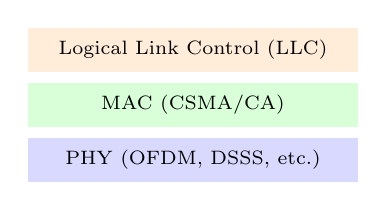
\begin{tikzpicture}[scale=0.7, every node/.style={font=\scriptsize}]
            \fill[blue!15] (0,0) rectangle (6,0.8);
            \node at (3,0.4) {PHY (OFDM, DSSS, etc.)};
            \fill[green!15] (0,1.0) rectangle (6,1.8);
            \node at (3,1.4) {MAC (CSMA/CA)};
            \fill[orange!15] (0,2.0) rectangle (6,2.8);
            \node at (3,2.4) {Logical Link Control (LLC)};
        \end{tikzpicture}
        \end{center}
        
        \vspace{0.2cm}
        \textbf{Key:} Wi-Fi defines layers 1 and 2 only. Everything above (IP, TCP, HTTP) runs on top unchanged.
    \end{columns}
\end{frame}

\begin{frame}{Wi-Fi Evolution: From 802.11b to Wi-Fi 7}
    \footnotesize
    \begin{center}
    \begin{tabular}{lcccccc}
        \toprule
        & \textbf{802.11b} & \textbf{802.11n} & \textbf{802.11ac} & \textbf{802.11ax} & \textbf{802.11ah} & \textbf{802.11be} \\
        & & \textbf{Wi-Fi 4} & \textbf{Wi-Fi 5} & \textbf{Wi-Fi 6/6E} & \textbf{HaLow} & \textbf{Wi-Fi 7} \\
        \midrule
        Year & 1999 & 2009 & 2013 & 2020 & 2017 & \textbf{2025} \\
        Freq. & 2.4 GHz & 2.4/5 & 5 GHz & 2.4/5/6 & \textbf{900 MHz} & 2.4/5/6 \\
        BW & 22 MHz & 20/40 & 20--160 & 20--160 & 1--16 & \textbf{20--320} \\
        Modulation & DSSS & OFDM & 256-QAM & 1024-QAM & OFDM & \textbf{4096-QAM} \\
        MIMO & --- & 4$\times$4 & MU-MIMO & MU-MIMO & MIMO & MU-MIMO \\
        Peak rate & 11 Mbps & 600 & 6933 & 9608 & 347 & \textbf{46,120} \\
        Key for IoT & Legacy & Common & --- & OFDMA & \textbf{Long range} & MLO \\
        \bottomrule
    \end{tabular}
    \end{center}
    \normalsize
    
    \vspace{0.2cm}
    \begin{columns}
        \column{0.5\textwidth}
        \begin{exampleblock}{802.11ah (HaLow) for IoT}
            900 MHz $\Rightarrow$ longer range (up to 1 km).
            All 802.11ac clocks scaled 10x slower.
            But: slow industry adoption.
        \end{exampleblock}
        
        \column{0.5\textwidth}
        \begin{alertblock}{Wi-Fi 7 (802.11be, July 2025)}
            Multi-Link Operation (MLO): use 2.4 + 5 + 6 GHz simultaneously.
            320 MHz channels, 4096-QAM.
            Lower latency for real-time IoT.
        \end{alertblock}
    \end{columns}
\end{frame}

\begin{frame}{Wi-Fi MAC: CSMA/CA and the Hidden Terminal Problem}
    \textbf{Wi-Fi uses CSMA/CA} (Collision Avoidance, not Detection):
    
    \begin{enumerate}
        \item \textbf{Listen} before transmitting (carrier sense)
        \item If channel busy, \textbf{back off} random time
        \item Transmit frame, wait for \textbf{ACK}
        \item No ACK $\Rightarrow$ assume collision, retry with larger backoff
    \end{enumerate}
    
    \vspace{0.2cm}
    \textbf{Why not Collision Detection (CSMA/CD)?}
    \begin{itemize}
        \item In wireless, a node \textbf{cannot listen while transmitting} (self-interference)
        \item So collisions are detected \textit{after the fact} via missing ACKs
    \end{itemize}
    
    \vspace{0.2cm}
    \textbf{Hidden Terminal $\Rightarrow$ RTS/CTS solution:}
    \begin{itemize}
        \item Node A and C can't hear each other, but both transmit to B $\Rightarrow$ collision at B
        \item \textbf{RTS/CTS:} A sends short Request-to-Send; B replies Clear-to-Send
        \item C hears CTS and defers (sets NAV timer = Network Allocation Vector)
        \item Overhead: 2 extra frames per data frame (not always worth it for small packets)
    \end{itemize}
\end{frame}

%==============================================================================
\section{Cellular IoT}
%==============================================================================

\begin{frame}{Cellular IoT: NB-IoT, LTE-M, and 5G RedCap}
    \footnotesize
    \begin{center}
    \begin{tabular}{lccccc}
        \toprule
        & \textbf{LTE Cat-1} & \textbf{LTE-M} & \textbf{NB-IoT} & \textbf{5G RedCap} & \textbf{5G eRedCap} \\
        & & \textbf{(Cat-M1)} & \textbf{(Cat-NB2)} & \textbf{(Rel-17)} & \textbf{(Rel-18, 2024)} \\
        \midrule
        DL rate & 10 Mbps & 1 Mbps & 127 kbps & 150 Mbps & 10 Mbps \\
        UL rate & 5 Mbps & 1 Mbps & 159 kbps & 50 Mbps & 5 Mbps \\
        Bandwidth & 20 MHz & 1.08 MHz & 180 kHz & 20 MHz & 5 MHz \\
        Latency & 10--15 ms & 10--15 ms & 1.6--10 s & 5 ms & 5 ms \\
        Antennas & 2 (MIMO) & 1 (SISO) & 1 (SISO) & 1--2 & 1 \\
        TX power & 23 dBm & 20/23 dBm & 20/23 dBm & 23 dBm & 20 dBm \\
        Mobility & Full & Full & Limited & Full & Limited \\
        Battery & Months & Years & \textbf{10+ years} & Months & \textbf{Years} \\
        \bottomrule
    \end{tabular}
    \end{center}
    \normalsize
    
    \vspace{0.2cm}
    \begin{alertblock}{5G RedCap and eRedCap (2024): Bridging the Gap}
        \textbf{RedCap} (Rel-17): Simplified 5G for wearables, video surveillance. Replaces LTE Cat-4.
        
        \textbf{eRedCap} (Rel-18, June 2024): Even simpler. 5 MHz BW, 1 antenna. Targets NB-IoT/LTE-M replacement with 5G NR access. Extended DRX for multi-year battery life.
    \end{alertblock}
\end{frame}

\begin{frame}{What Does Everyone Else Use?}
    \textbf{Popular consumer IoT devices and their connectivity:}
    
    \vspace{0.3cm}
    \begin{center}
    \begin{tabular}{lll}
        \toprule
        \textbf{Device} & \textbf{Protocol} & \textbf{Why?} \\
        \midrule
        Amazon Echo & Wi-Fi + BLE + Zigbee + Thread & Hub for all ecosystems \\
        Google Nest & Wi-Fi + Thread + Matter & Thread border router \\
        Philips Hue & Zigbee (+ Matter bridge) & Legacy mesh, migrating \\
        Ring Doorbell & Wi-Fi (video) + Z-Wave (sensors) & High bandwidth for video \\
        Apple HomePod & Wi-Fi + Thread + Matter & Thread border router \\
        Smart plugs/bulbs & Wi-Fi or Thread/Matter & Cost-driven choice \\
        \bottomrule
    \end{tabular}
    \end{center}
    
    \vspace{0.3cm}
    \begin{exampleblock}{Trend (2024--2025)}
        Consumer IoT is converging on \textbf{Matter over Thread} (low power mesh) and \textbf{Matter over Wi-Fi} (high bandwidth). BLE used for commissioning (onboarding new devices).
    \end{exampleblock}
\end{frame}

%==============================================================================
\section{LPWAN Technologies}
%==============================================================================

\begin{frame}{The LPWAN Sweet Spot}
    \textbf{Classical technologies left a gap:}
    
    \vspace{0.2cm}
    \begin{columns}
        \column{0.5\textwidth}
        \textbf{Group 1 (Short Range):}
        \begin{itemize}
            \item RFID, 802.15.4, Bluetooth, Wi-Fi
            \item Low cost, low power
            \item But: tens to hundreds of meters only
            \item Need local coordinator (AP, hub, phone)
        \end{itemize}
        
        \vspace{0.2cm}
        \textbf{Group 2 (Cellular WAN):}
        \begin{itemize}
            \item 3G/4G/5G
            \item Kilometers of range
            \item But: expensive devices (complex protocols)
            \item Monthly subscription cost
        \end{itemize}
        
        \column{0.5\textwidth}
        \begin{alertblock}{The LPWAN Gap}
            \textbf{Low cost} + \textbf{low power} + \textbf{long range}
            
            \vspace{0.2cm}
            Sacrifice: \textbf{data rate} (kbps, not Mbps)
            
            \vspace{0.2cm}
            For most IoT sensors, this is perfectly acceptable---a soil moisture reading is 2 bytes!
        \end{alertblock}
        
        \vspace{0.2cm}
        \textbf{LPWAN properties:}
        \begin{itemize}
            \item Base-station infrastructure
            \item Simple PHY/MAC (like early Wi-Fi)
            \item Unlicensed OR licensed spectrum
            \item kbps data rates
            \item km range
        \end{itemize}
    \end{columns}
\end{frame}

\begin{frame}{LoRaWAN: Physical Layer -- Chirp Spread Spectrum}
    \textbf{LoRa uses Chirp Spread Spectrum (CSS) modulation:}
    
    \vspace{0.2cm}
    \begin{columns}
        \column{0.55\textwidth}
        \begin{itemize}
            \item A \textbf{chirp} is a signal whose frequency sweeps linearly
            \item Each symbol encodes \textbf{SF bits} by starting the chirp at a different frequency offset
            \item Symbol time: $T_s = 2^{SF} / BW$
            \item More spreading $\Rightarrow$ longer symbol $\Rightarrow$ more robust $\Rightarrow$ slower
        \end{itemize}
        
        \vspace{0.2cm}
        \textbf{Why CSS?}
        \begin{itemize}
            \item Resilient to narrowband interference
            \item Resilient to multipath fading
            \item Resilient to Doppler shift
            \item Simple receiver (FFT of dechirped signal)
        \end{itemize}
        
        \column{0.45\textwidth}
        \textbf{Key formulas:}
        
        \vspace{0.2cm}
        Symbol rate:
        \[ R_s = \frac{BW}{2^{SF}} \]
        
        Bit rate:
        \[ R_b = SF \times \frac{BW}{2^{SF}} \]
        
        \vspace{0.2cm}
        Example (SF7, BW=125kHz):
        \[ R_b = 7 \times \frac{125000}{128} = 5470 \text{ bps} \]
        
        Example (SF12, BW=125kHz):
        \[ R_b = 12 \times \frac{125000}{4096} = 366 \text{ bps} \]
    \end{columns}
\end{frame}

\begin{frame}{LoRa Spreading Factors: The Fundamental Tradeoff}
    \begin{center}
    \begin{tabular}{cccccc}
        \toprule
        \textbf{SF} & \textbf{BW} & \textbf{Bit Rate} & \textbf{Sensitivity} & \textbf{Airtime} & \textbf{Range} \\
        & & \textbf{(bps)} & \textbf{(dBm)} & \textbf{(11B pkt)} & \textbf{(approx)} \\
        \midrule
        7 & 125 kHz & 5,470 & $-123$ & 41 ms & 2 km \\
        8 & 125 kHz & 3,125 & $-126$ & 72 ms & 3 km \\
        9 & 125 kHz & 1,760 & $-129$ & 144 ms & 5 km \\
        10 & 125 kHz & 980 & $-132$ & 288 ms & 8 km \\
        11 & 125 kHz & 440 & $-134.5$ & 577 ms & 11 km \\
        12 & 125 kHz & 250 & $-137$ & 1,155 ms & 15 km \\
        \bottomrule
    \end{tabular}
    \end{center}
    
    \vspace{0.2cm}
    \begin{columns}
        \column{0.5\textwidth}
        \begin{alertblock}{Tradeoff}
            Each SF step: +3 dB sensitivity ($\approx$ 2x range) but 2x airtime $\Rightarrow$ 2x energy and half the throughput.
        \end{alertblock}
        
        \column{0.5\textwidth}
        \begin{exampleblock}{Orthogonality}
            Different SFs are \textbf{quasi-orthogonal}: gateway can receive SF7 and SF12 simultaneously on the same frequency!
        \end{exampleblock}
    \end{columns}
\end{frame}

\begin{frame}{LoRaWAN: Device Classes}
    \begin{columns}
        \column{0.33\textwidth}
        \textbf{Class A} (all devices):
        \begin{itemize}
            \item Bidirectional
            \item Device initiates uplink
            \item 2 short RX windows after TX
            \item \textbf{Lowest power}
            \item Best for: sensors
        \end{itemize}
        
        \vspace{0.2cm}
        \begin{center}
        \scriptsize
        TX $\rightarrow$ RX1 $\rightarrow$ RX2 $\rightarrow$ sleep
        \normalsize
        \end{center}
        
        \column{0.33\textwidth}
        \textbf{Class B} (scheduled):
        \begin{itemize}
            \item Class A + periodic ping slots
            \item Gateway sends beacon for sync
            \item Server can schedule downlinks
            \item \textbf{Medium power}
            \item Best for: actuators
        \end{itemize}
        
        \vspace{0.2cm}
        \begin{center}
        \scriptsize
        BCN $\rightarrow$ PNG $\rightarrow$ TX $\rightarrow$ RX1 $\rightarrow$ RX2
        \normalsize
        \end{center}
        
        \column{0.33\textwidth}
        \textbf{Class C} (continuous):
        \begin{itemize}
            \item Always listening (RX2 open)
            \item Server can send anytime
            \item No latency for downlink
            \item \textbf{Highest power}
            \item Best for: mains-powered
        \end{itemize}
        
        \vspace{0.2cm}
        \begin{center}
        \scriptsize
        RX2 $\rightarrow$ TX $\rightarrow$ RX1 $\rightarrow$ RX2 (always)
        \normalsize
        \end{center}
    \end{columns}
    
    \vspace{0.3cm}
    \begin{alertblock}{LoRaWAN 1.0.4 (2023) -- New: Relay}
        TS011: End-devices can relay frames for other devices, extending coverage without additional gateways. Useful for deep-indoor or underground sensors.
    \end{alertblock}
\end{frame}

\begin{frame}{LoRaWAN: Security and Scalability}
    \begin{columns}
        \column{0.5\textwidth}
        \textbf{Two-layer AES-128 security:}
        
        \vspace{0.2cm}
        \textbf{1. Network Session Key (NwkSKey):}
        \begin{itemize}
            \item Shared: end-device $\leftrightarrow$ network server
            \item Authenticates node in network
            \item Message Integrity Check (MIC)
        \end{itemize}
        
        \vspace{0.2cm}
        \textbf{2. Application Session Key (AppSKey):}
        \begin{itemize}
            \item Shared: end-device $\leftrightarrow$ app server
            \item Encrypts application payload
            \item Network operator \textbf{cannot} read data
        \end{itemize}
        
        \column{0.5\textwidth}
        \textbf{Scalability mechanisms:}
        \begin{itemize}
            \item Gateways listen on 8 frequencies
            \item All SFs per frequency (concurrent!)
            \item \textbf{Adaptive Data Rate (ADR):}
            \begin{itemize}
                \item Server tells device to use lowest SF possible
                \item Closer to gateway $\Rightarrow$ lower SF $\Rightarrow$ more capacity
            \end{itemize}
            \item Congestion $\Rightarrow$ add gateways
            \begin{itemize}
                \item Nodes get closer to a gateway
                \item ADR reduces SF
                \item Capacity scales multiplicatively!
            \end{itemize}
        \end{itemize}
    \end{columns}
    
    \vspace{0.2cm}
    \begin{exampleblock}{Key: End-to-end encryption separates network from application}
        The network operator routes packets but cannot decrypt your sensor data. This is crucial for privacy-sensitive IoT deployments.
    \end{exampleblock}
\end{frame}

\begin{frame}{Sigfox / 0G Technology}
    \begin{columns}
        \column{0.5\textwidth}
        \textbf{Ultra-Narrowband (UNB) approach:}
        \begin{itemize}
            \item 100 Hz channels (vs 125 kHz for LoRa!)
            \item Randomly placed within 200 kHz band
            \item ISM band (same as LoRaWAN)
        \end{itemize}
        
        \vspace{0.2cm}
        \textbf{Physical layer:}
        \begin{itemize}
            \item Uplink: 100 bps (DBPSK)
            \item Downlink: 600 bps (GFSK)
            \item 12-byte packets, 3x repetition
            \item Max 140 uplink messages/day
        \end{itemize}
        
        \vspace{0.2cm}
        \textbf{Architecture:}
        \begin{itemize}
            \item Gateways and cloud managed by operator
            \item Very simple end-devices (no MAC state)
        \end{itemize}
        
        \column{0.5\textwidth}
        \textbf{Status (2024--2025):}
        \begin{itemize}
            \item Original Sigfox: bankrupt 2022
            \item Acquired by \textbf{UnaBiz}
            \item Rebranded as \textbf{``0G Technology''}
            \item 14+ million connected devices
            \item 75+ countries network coverage
        \end{itemize}
        
        \vspace{0.2cm}
        \textbf{2024 update:}
        \begin{itemize}
            \item \textbf{Sub0G program:} ultra-low-cost tracking
            \item 18x energy reduction (new protocol optimizations)
            \item Focus: supply chain, logistics
        \end{itemize}
        
        \vspace{0.2cm}
        \begin{alertblock}{UNB vs CSS}
            Sigfox: simpler device, operator-managed.
            LoRaWAN: more flexible, private networks possible.
        \end{alertblock}
    \end{columns}
\end{frame}

%==============================================================================
\section{Technology Classification}
%==============================================================================

\begin{frame}{Technology Classification: The Big Picture}
    \begin{center}
    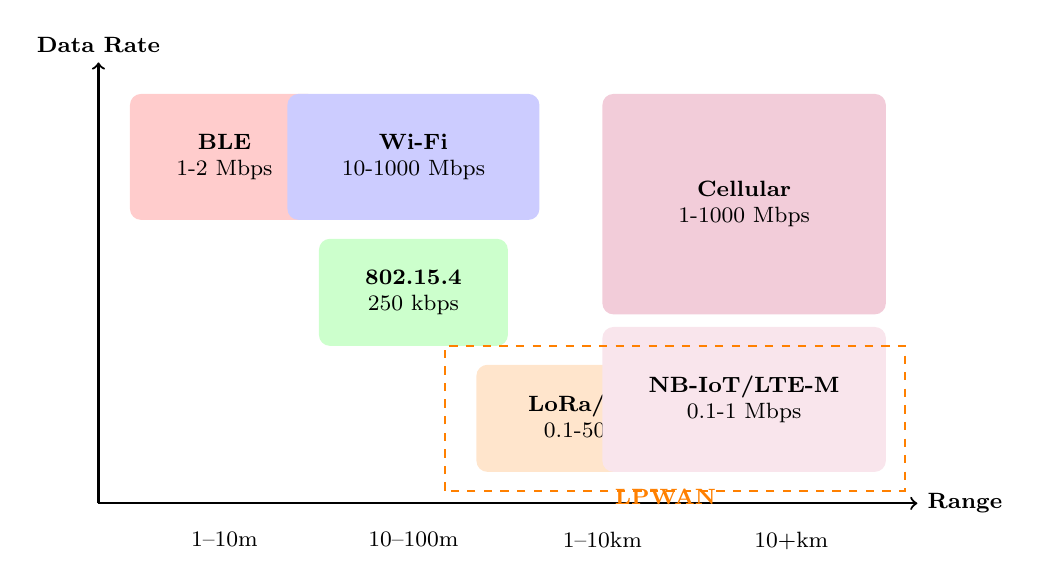
\begin{tikzpicture}[scale=0.8, every node/.style={font=\footnotesize}]
        % Axes
        \draw[->, thick] (0,0) -- (13,0) node[right] {\textbf{Range}};
        \draw[->, thick] (0,0) -- (0,7) node[above] {\textbf{Data Rate}};
        % Labels
        \node[below] at (2,-0.3) {1--10m};
        \node[below] at (5,-0.3) {10--100m};
        \node[below] at (8,-0.3) {1--10km};
        \node[below] at (11,-0.3) {10+km};
        % Bubbles
        \fill[red!20, rounded corners] (0.5,4.5) rectangle (3.5,6.5);
        \node[align=center] at (2,5.5) {\textbf{BLE}\\1-2 Mbps};
        \fill[blue!20, rounded corners] (3,4.5) rectangle (7,6.5);
        \node[align=center] at (5,5.5) {\textbf{Wi-Fi}\\10-1000 Mbps};
        \fill[green!20, rounded corners] (3.5,2.5) rectangle (6.5,4.2);
        \node[align=center] at (5,3.35) {\textbf{802.15.4}\\250 kbps};
        \fill[orange!20, rounded corners] (6,0.5) rectangle (10,2.2);
        \node[align=center] at (8,1.35) {\textbf{LoRa/Sigfox}\\0.1-50 kbps};
        \fill[purple!20, rounded corners] (8,3.0) rectangle (12.5,6.5);
        \node[align=center] at (10.25,4.75) {\textbf{Cellular}\\1-1000 Mbps};
        \fill[purple!10, rounded corners] (8,0.5) rectangle (12.5,2.8);
        \node[align=center] at (10.25,1.65) {\textbf{NB-IoT/LTE-M}\\0.1-1 Mbps};
        % LPWAN label
        \draw[dashed, thick, orange] (5.5,0.2) rectangle (12.8,2.5);
        \node[orange, font=\footnotesize\bfseries] at (9,0.1) {LPWAN};
    \end{tikzpicture}
    \end{center}
    
    \vspace{0.1cm}
    \begin{exampleblock}{No single technology covers all IoT needs}
        The protocol selection depends on your \textbf{dominant constraint}: range, data rate, power, cost, or latency. Use the elimination method from the practical exercises.
    \end{exampleblock}
\end{frame}

\begin{frame}{LoRaWAN vs Sigfox vs NB-IoT: Head-to-Head}
    \begin{center}
    \begin{tabular}{lccc}
        \toprule
        & \textbf{LoRaWAN} & \textbf{Sigfox (0G)} & \textbf{NB-IoT} \\
        \midrule
        Spectrum & Unlicensed (ISM) & Unlicensed (ISM) & Licensed (cellular) \\
        Modulation & CSS (LoRa) & UNB (DBPSK) & OFDMA \\
        UL rate & 0.3--50 kbps & 100 bps & 127 kbps \\
        DL rate & 0.3--50 kbps & 600 bps & 159 kbps \\
        Payload & 242 bytes & 12 bytes & 1600 bytes \\
        Messages/day & Unlimited (duty cycle) & 140 UL, 4 DL & Unlimited \\
        Private network & \textbf{Yes} & No (operator only) & No (operator only) \\
        Range (rural) & 10--15 km & 30--50 km & 10--15 km \\
        Battery life & 5--10 years & 5--10 years & 10+ years (PSM) \\
        Cost/device & \$3--8 (module) & \$2--5 (module) & \$5--10 (module) \\
        Subscription & Free (private) & \$1--2/yr & \$1--5/yr \\
        \bottomrule
    \end{tabular}
    \end{center}
    
    \vspace{0.2cm}
    \begin{alertblock}{Decision Guide}
        \textbf{LoRaWAN:} You want control (private network), moderate payload, bidirectional.
        \textbf{Sigfox:} Ultra-simple, tiny payloads, massive scale, operator-managed.
        \textbf{NB-IoT:} Need guaranteed QoS, larger payloads, cellular coverage, no gateway to deploy.
    \end{alertblock}
\end{frame}

%==============================================================================
\section{Summary}
%==============================================================================

\begin{frame}{Key Takeaways}
    \begin{columns}
        \column{0.5\textwidth}
        \textbf{Short-Range Standards:}
        \begin{itemize}
            \item \textbf{802.15.4:} Foundation for ZigBee, Thread, Matter. Beacon superframe enables GTS.
            \item \textbf{Bluetooth/BLE:} Piconet/TDMA for classic; advertising/connection for BLE. BT 6.0 adds cm-level ranging.
            \item \textbf{Wi-Fi:} CSMA/CA, high throughput. 802.11ah for IoT range. Wi-Fi 7 for low-latency MLO.
        \end{itemize}
        
        \column{0.5\textwidth}
        \textbf{Long-Range Standards:}
        \begin{itemize}
            \item \textbf{LoRaWAN:} CSS modulation, SF tradeoff (range vs rate), 3 device classes, 2-layer security.
            \item \textbf{Sigfox/0G:} Ultra-narrowband, simplest device, but limited payload and messages.
            \item \textbf{Cellular IoT:} NB-IoT for static low-rate; LTE-M for mobile; 5G RedCap bridging the gap.
        \end{itemize}
    \end{columns}
    
    \vspace{0.3cm}
    \begin{alertblock}{The Meta-Lesson}
        Standards evolve fast---Matter 1.5, BT 6.1, Wi-Fi 7, 5G eRedCap all arrived in 2024--2025. As an engineer, \textbf{check the latest specs}, not textbook tables from 3 years ago.
    \end{alertblock}
\end{frame}

\begin{frame}{Questions?}
    \begin{center}
        \Huge Questions?
        
        \vspace{1cm}
        \normalsize
        \textbf{Eduardo Baena}\\
        \texttt{e.baena@northeastern.edu}
        
        \vspace{0.5cm}
        \textit{EECE5155: Wireless Sensor Networks and the Internet of Things}\\
        Spring 2026
    \end{center}
\end{frame}

\end{document}
